\documentclass[tikz]{standalone}
\usetikzlibrary{automata, positioning, arrows.meta}

\begin{document}
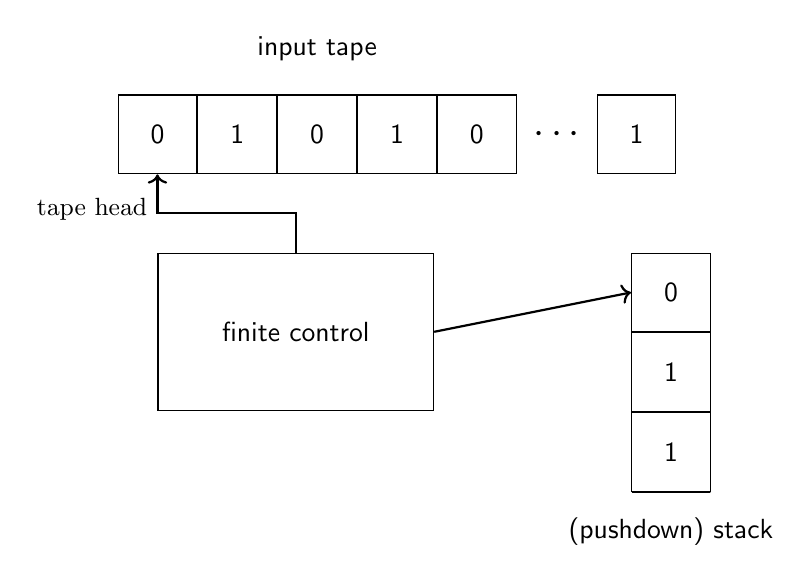
\begin{tikzpicture}[
every node/.style={font=\sffamily},
tape cell/.style={draw, minimum width=1cm, minimum height=1cm},
stack box/.style={draw, minimum width=1cm, minimum height=1cm, align=center},
arrow/.style={->, thick},
]

% Finite control box
\node[draw, minimum width=3.5cm, minimum height=2cm, align=center] (fc) {finite control};

% Tape above the finite control
\node[tape cell, above=2cm of fc.west, xshift=0cm] (t1) {0};
\node[tape cell, right=0cm of t1] (t2) {1};
\node[tape cell, right=0cm of t2] (t3) {0};
\node[tape cell, right=0cm of t3] (t4) {1};
\node[tape cell, right=0cm of t4] (t5) {0};
\node[minimum width=1cm, minimum height=1cm, right=0cm of t5] (dots) {\Large$\cdots$};
\node[tape cell, right=0cm of dots] (t6) {1};

% Label above the tape
\node[above=0.3cm of t3] {input tape};

% Arrow from FC to tape head with label
\draw[arrow] 
  (fc.north) -- ++(0,0.5) 
  -| node[pos=0.55, left, font=\small] {tape head} (t1.south);

% Stack to the right of FC
\node[stack box, right=2.5cm of fc.north east, anchor=north west] (s1) {0};
\node[stack box, below=0cm of s1] (s2) {1};
\node[stack box, below=0cm of s2] (s3) {1};

% Stack base (triangle base)
\draw ([xshift=-0.5cm]s3.south) -- ++(1cm,0) -- ([xshift=-0.5cm]s3.south);

% Arrow from FC to stack
\draw[arrow] (fc.east) -- (s1.west);

% Label for stack
\node[below=0.2cm of s3] {(pushdown) stack};
\end{tikzpicture}
\end{document}
